% This LaTeX was auto-generated from MATLAB code.
% To make changes, update the MATLAB code and export to LaTeX again.

\documentclass{article}

\usepackage[utf8]{inputenc}
\usepackage[T1]{fontenc}
\usepackage{lmodern}
\usepackage{graphicx}
\usepackage{color}
\usepackage{hyperref}
\usepackage{amsmath}
\usepackage{amsfonts}
\usepackage{epstopdf}
\usepackage[table]{xcolor}
\usepackage{matlab}
\usepackage[paperheight=795pt,paperwidth=614pt,top=72pt,bottom=72pt,right=72pt,left=72pt,heightrounded]{geometry}

\sloppy
\epstopdfsetup{outdir=./}
\graphicspath{ {./findPVCs_media/} }

\begin{document}

\matlabtitle{LAB SESSION 1: INTRODUCTION TO SIGNAL PROCESSING}

\matlabheading{Biomedical Signals}

\matlabheadingthree{\underline{\textbf{Student Names:}}\textbf{ Marta Maldonado and Marcos Oriol}}


\vspace{1em}

\vspace{1em}
\begin{matlabcode}
% Load data
addpath('routines/');

% Visualize ECG along time using command 'visualpvc'
load("data/ecgpvc.mat");
%visualpvc(ecgpvc);
\end{matlabcode}


\vspace{1em}

\matlabheading{1. Detecting PVC}

\begin{par}
\begin{flushleft}
In this section, an ECG signal with premature ventricular contractions (PVC) will be analyzed in order to detect the ectopic beats by using cross-correlation function.
\end{flushleft}
\end{par}

\begin{par}
\begin{flushleft}
\underline{Objective:} detect automatically the ectopic beats using normalized cross-correation between the ECG signal and a 'representative' ectopic beat pattern.
\end{flushleft}
\end{par}

\matlabheadingthree{\textbf{1.1. Representative Ectopic Beat Pattern}}

\begin{par}
\begin{flushleft}
This representative ectopic beat is built using the average of five ectopic beats. For this purpose, we have first detected 5 ectopic beats, which we are going to work on. Then, we have selected the time when the maximum value (corresponding to the R wave) appears, for each of the five selected beats, as can be seen in the following image:
\end{flushleft}
\end{par}

\begin{par}
\begin{flushleft}
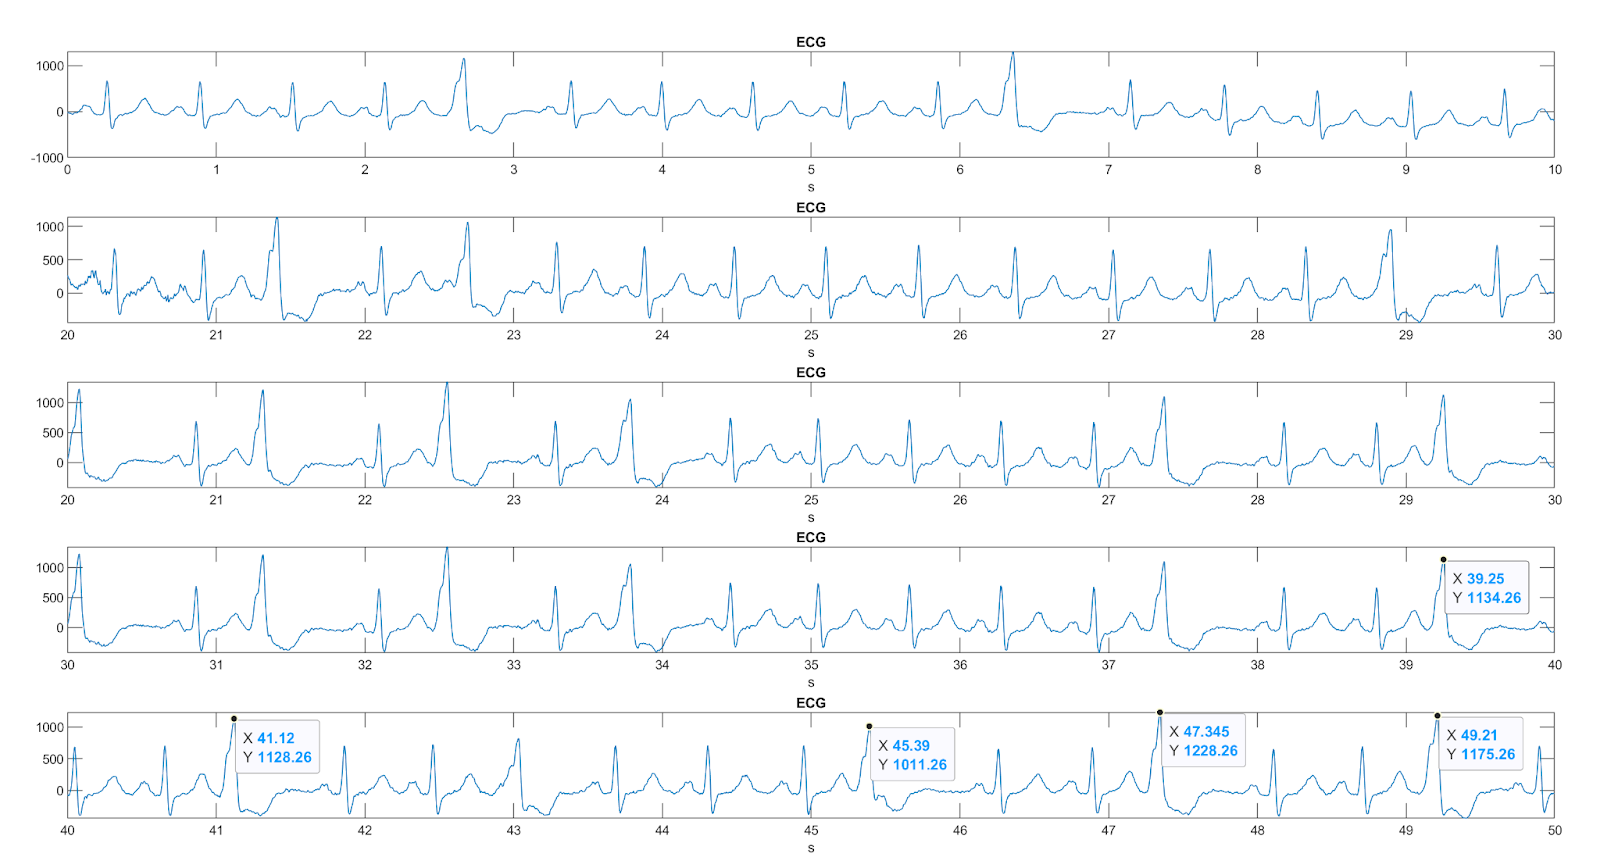
\includegraphics[width=\maxwidth{60.41144004014049em}]{image_0}
\end{flushleft}
\end{par}

\begin{par}
\begin{flushleft}
Then, we have fixed a sample window around the R wave, which includes the P and T waves of the beat.
\end{flushleft}
\end{par}

\begin{matlabcode}
% Manually take the time of the R wave of 5 ectopic beats
peaks = [39.25, 41.12, 45.39,47.345 ,49.1 ];

% Parameters
fs = 200; % Sampling frequency
peak_samples = peaks * fs;
sample_window = 50; % window

% Extract a windor cenetered around the selected peaks
window_accum_values = zeros(sample_window*2, 1);
for i = peak_samples
    window = ecgpvc(i-sample_window:i+sample_window-1);
    window_accum_values = window_accum_values + window;
end

% Average of all detected ectopic beats
representative_beat = window_accum_values / length(peak_samples);

figure;
plot(representative_beat);
title('Representative Ectopic Beat Pattern');
xlabel('Samples');
ylabel('Amplitude (mV)');
grid on;
\end{matlabcode}
\begin{center}
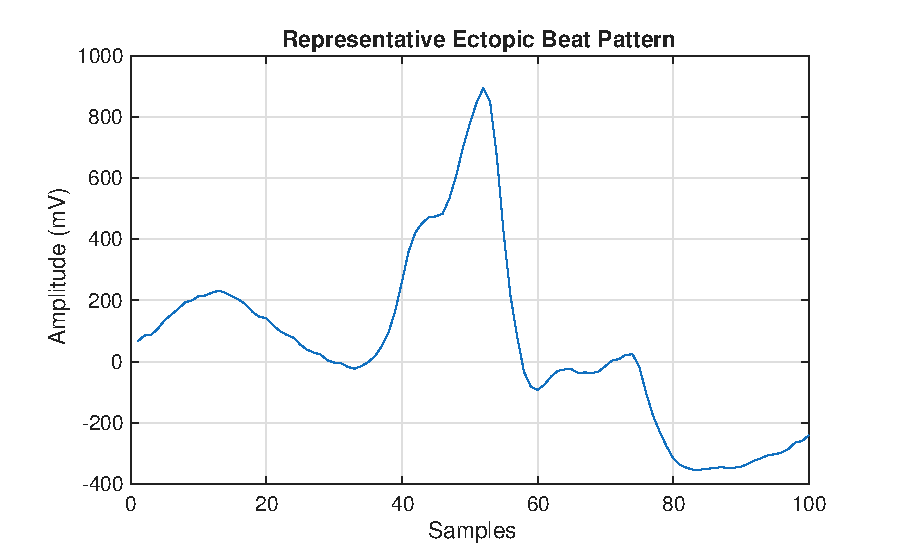
\includegraphics[width=\maxwidth{56.196688409433015em}]{figure_0.eps}
\end{center}


\vspace{1em}
\begin{par}
\begin{flushleft}
\textbf{1.2. Normalized Cross-Correlation}
\end{flushleft}
\end{par}

\begin{par}
\begin{flushleft}
Once we have calculated the pattern of the representative ectopic ECG beat, we now need to:
\end{flushleft}
\end{par}

\begin{itemize}
\setlength{\itemsep}{-1ex}
   \item{\begin{flushleft} Apply 'xcorr' between the ECG signal and the representative ectopic beat, to compute their similarity at each lag. \end{flushleft}}
   \item{\begin{flushleft} Normalization. \end{flushleft}}
\end{itemize}

\begin{matlabcode}
% Cross-correlation between 'ecgpvc' and 'representative_beat'
[corr, lags] = xcorr(ecgpvc, representative_beat);

% Since the full cross-correlation is symmetric, we keep the positive lags
trimmed_corr = corr(lags >= 0);

% Normalization
normalized_trim_corr = trimmed_corr / max(trimmed_corr);

figure;
plot(normalized_trim_corr);
title('Normalized Cross-Correlation between ECG and Rep. Ectopic Beat');
xlabel('Lag (samples)');
ylabel('Normalized Correlation');
ylim([0 1]);
grid on;
\end{matlabcode}
\begin{center}
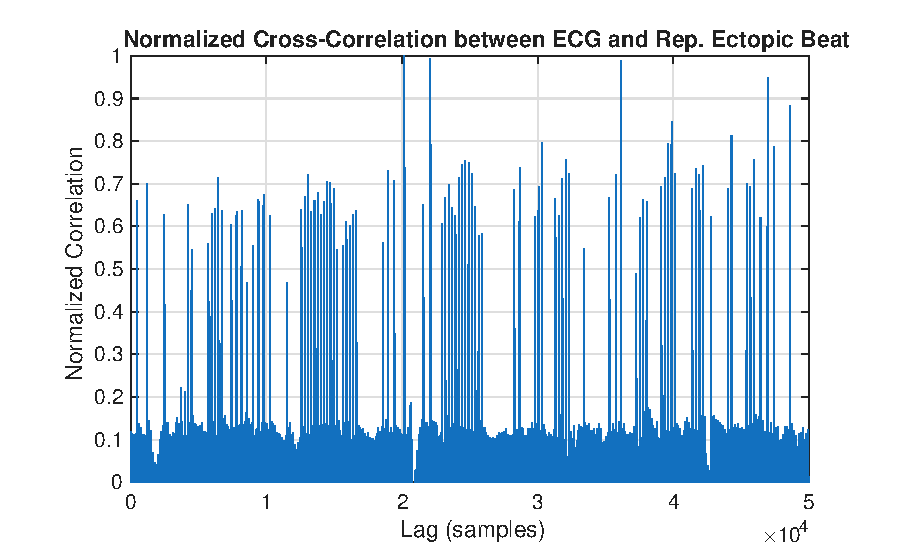
\includegraphics[width=\maxwidth{56.196688409433015em}]{figure_1.eps}
\end{center}


\vspace{1em}
\begin{par}
\begin{flushleft}
\textbf{1.3. Apply a threshold}
\end{flushleft}
\end{par}

\begin{par}
\begin{flushleft}
We now need to stablish a threshold in order to detect ectopic and normal beats. For this purpose, we have used two different methods:
\end{flushleft}
\end{par}

\begin{itemize}
\setlength{\itemsep}{-1ex}
   \item{\begin{flushleft} \textit{islocalmax} function in Matlab \end{flushleft}}
   \item{\begin{flushleft} \textit{findpeaks} function in Matlab \end{flushleft}}
\end{itemize}

\begin{par}
\begin{flushleft}
We are going to use both methods, for the later comparison of the number of ectopic beats detected with each of them.
\end{flushleft}
\end{par}

\begin{par}
\begin{flushleft}
     A) \underline{\textit{islocalmax}}
\end{flushleft}
\end{par}

\begin{matlabcode}
% Define the time knowing that the ECG signal was recorded during 250 seconds
record_duration = 250;
time = linspace(0, record_duration, 50000);

% Apply a threshold
threshold = 0.4;

% Find indxs above the threshold
idxs = find(normalized_trim_corr >= threshold);

% Find local maximum values of idxs
center_idx = find(islocalmax(normalized_trim_corr(idxs)) == 1);
max_samples = idxs(center_idx);
plot_local_max(ecgpvc, time, max_samples);
title("ECG and Detected Representative Ectopic Beats - 'islocalmax'");
xlabel('Time (s)');
ylabel('Amplitude (mV)');
\end{matlabcode}
\begin{center}
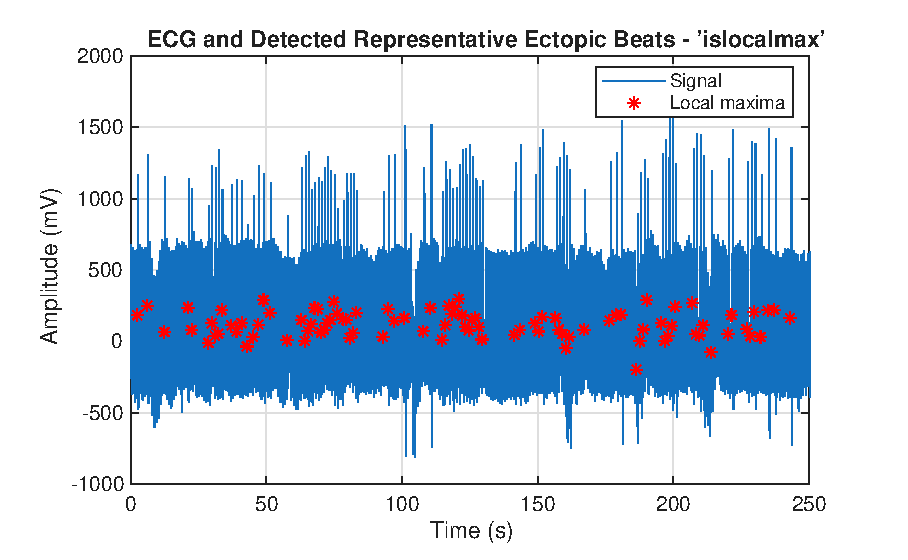
\includegraphics[width=\maxwidth{56.196688409433015em}]{figure_2.eps}
\end{center}

\begin{par}
\begin{flushleft}
In order to select the best threshold for detecting most of the ectopic beats present in the ECG signal, we tested different values while observing the resulting graph, similar to the one shown above with the ectopic beats marked with a red asterisk, in order to visually verify whether most of the ectopic beats were detected or not. After testing several threshold, we finally chose a \textbf{threshold of 0.4}, as almost all ectopic beats were detected, which we were able to verify by cosely inspecting the resulting graph obtained (the one shown above). With this configuration, a total of \textbf{92 ectopic beats} were detected.
\end{flushleft}
\end{par}

\begin{par}
\begin{flushleft}
If we look more closely at the final graph obtained (shown above) and zoom in (graph below), we can see that the red markers indicating the detected ectopic beats do not align exactly with the peaks of the ECG signal. This is because of how the cross-correlation function works, as the lag value obtained from this function representes where the start of the representative beat aligns with the ECG signal, but not the true peak of the ectopic beat. Therefore, since we have chosen a window that includes the P and T waves, we know that the R wave will lie within this window, not at the start of it. Consequently, although the red markers do not correspond precisely to the R wave, they indicate that an ectopic beat occurs close to each marker position.
\end{flushleft}
\end{par}

\begin{par}
\begin{flushleft}
                                         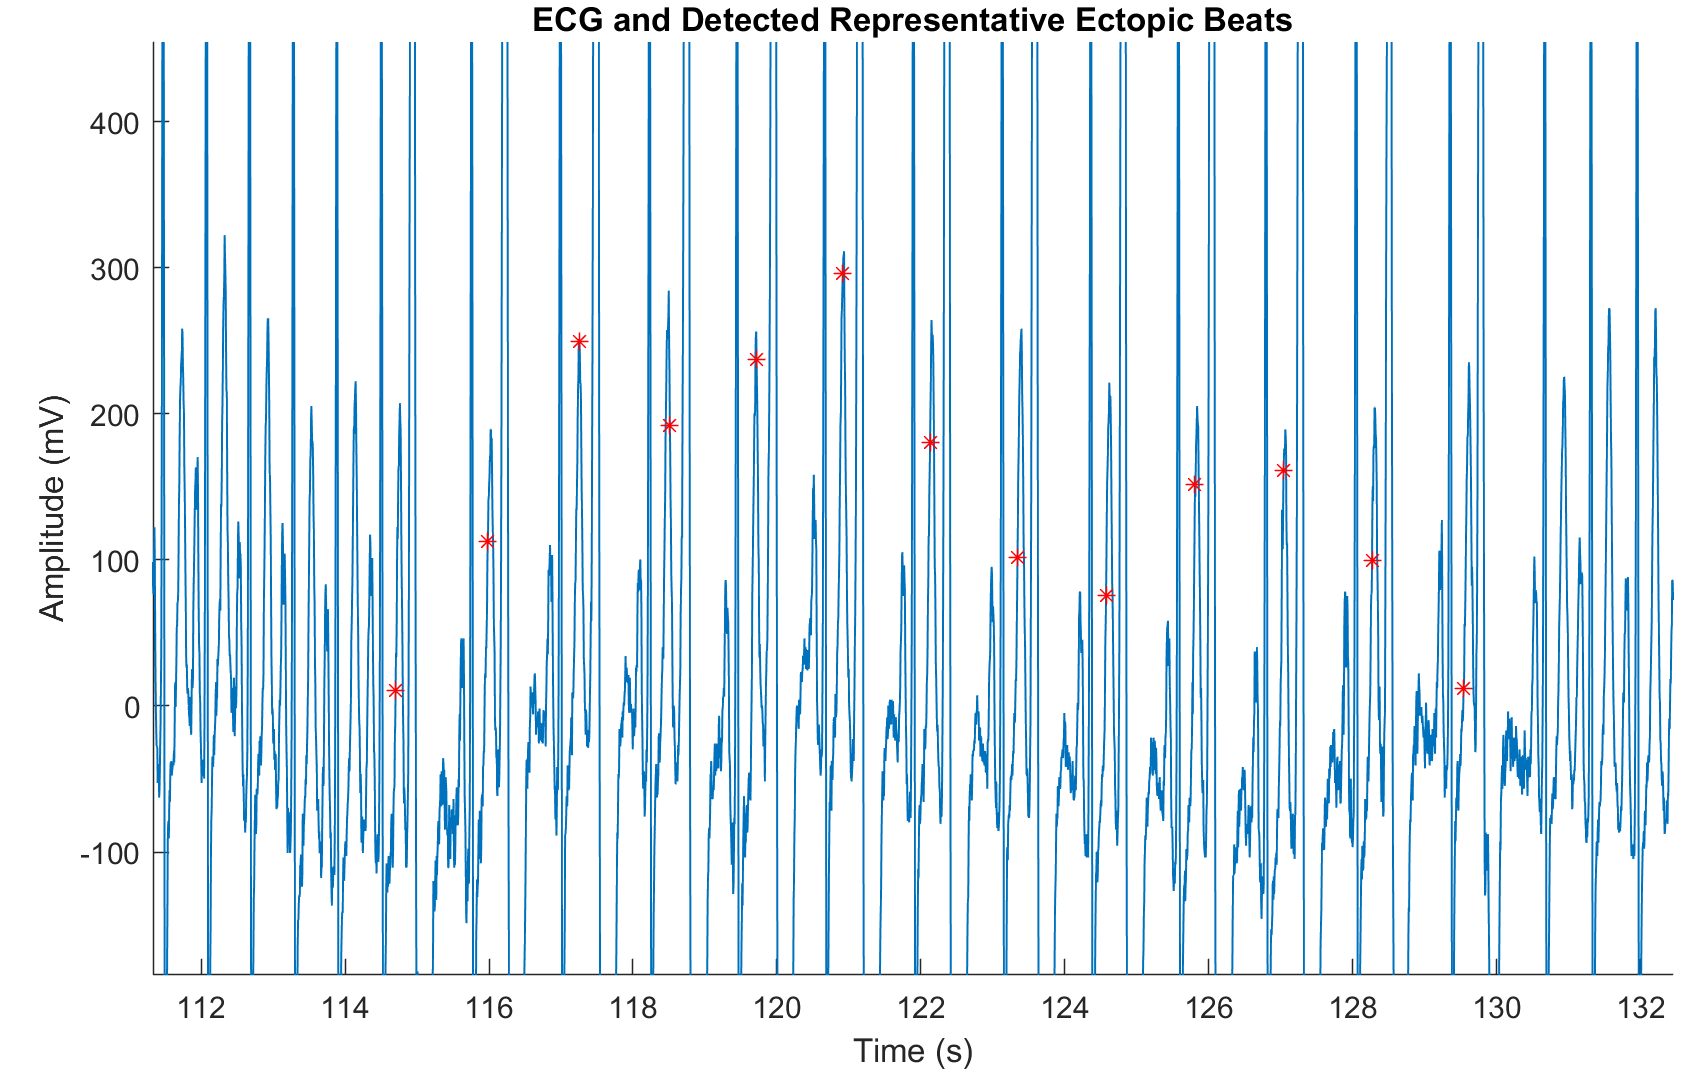
\includegraphics[width=\maxwidth{50.376317109884596em}]{image_1}
\end{flushleft}
\end{par}


\vspace{1em}
\begin{par}
\begin{flushleft}
     B) \underline{\textit{findpeaks:}}
\end{flushleft}
\end{par}

\begin{matlabcode}
% Apply a threshold
threshold = 0.4; 

% Find indxs above the threshold
[~, idxs] = findpeaks(normalized_trim_corr, "MinPeakHeight", 0.4);

% Plot the detected ectopic beats
plot_local_max(ecgpvc, time, idxs);
title("ECG and Detected Representative Ectopic Beats - 'findpeaks'");
xlabel('Time (s)');
ylabel('Amplitude (mV)');
\end{matlabcode}
\begin{center}
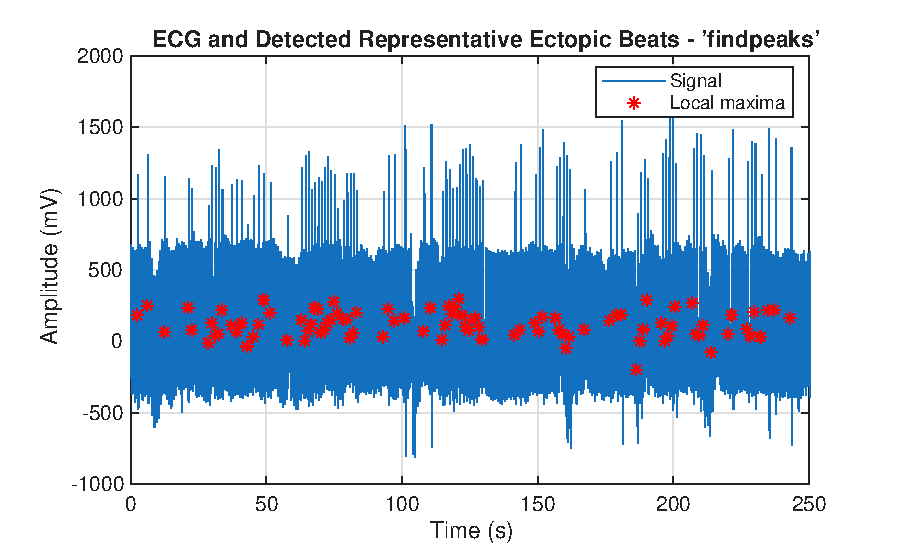
\includegraphics[width=\maxwidth{56.196688409433015em}]{figure_3.eps}
\end{center}

\begin{par}
\begin{flushleft}
It can be observed that with this second method we are detecting the same number of ectopic beats: \textbf{92 ectopic beats}.
\end{flushleft}
\end{par}


\matlabheading{2. Filtering ECG}

\matlabheadingtwo{2.1. Load the data and show it needs to be filtered.}

\begin{matlabcode}
clear all;
clc;

load("data/ecgf.mat");
fs = 1000; %Hz

\end{matlabcode}

\matlabheadingtwo{Plot the data}

\begin{matlabcode}
time = linspace(0, length(ecgf)/fs, length(ecgf));

figure;
plot(time, ecgf);
xlabel('Time (s)');
ylabel('Amplitude (mV)');
title('ECG along time');
\end{matlabcode}
\begin{center}
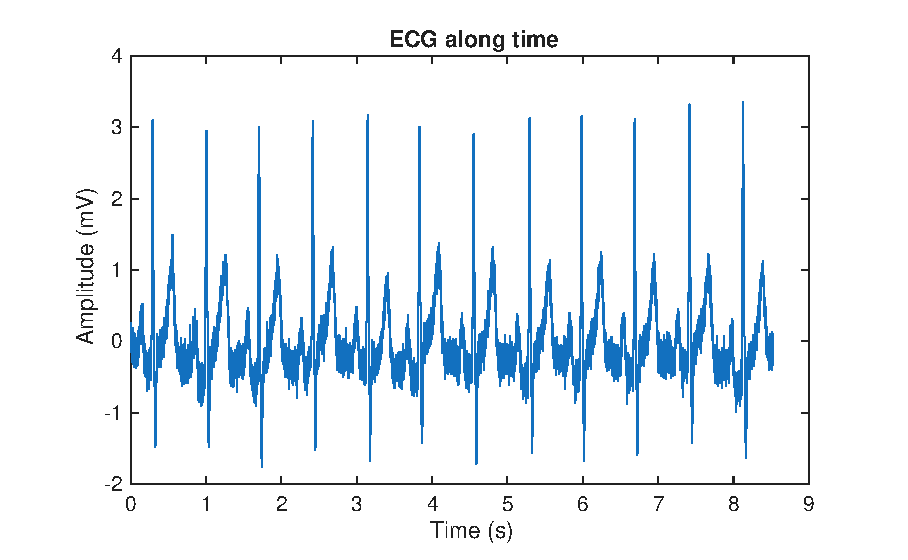
\includegraphics[width=\maxwidth{56.196688409433015em}]{figure_4.eps}
\end{center}

\begin{par}
\begin{flushleft}
As it can be seen, the signal has some noise that needs to be filtered. (high frequency oscillations surrounding the trend).
\end{flushleft}
\end{par}

\matlabheadingtwo{2.2. PSD and filter selection}

\begin{par}
\begin{flushleft}
In order to detect the noise that is affecting our signal, we will apply the fft algorithm and observe which are the major frequencies present. As we know which are the phisiological heart peak frequencies present in the ECG, we can determine which peaks are physiological, and which ones are from the noise.
\end{flushleft}
\end{par}

\begin{matlabcode}
% Compute FFT magnitude spectrum
[magnitude, f] = magnitude_spectrum(ecgf, fs);

% Compute PSD using Welch's method
[pxx, f_psd] = pwelch(ecgf, [], [], [], fs);

% Plot both in subplots
figure;

% FFT Magnitude
subplot(2,1,1);
plot(f, magnitude);
xlabel('Frequency (Hz)');
ylabel('Magnitude');
title('Magnitude Spectrum');

% PSD
subplot(2,1,2);
plot(f_psd, 10*log10(pxx));  % PSD in dB/Hz
xlabel('Frequency (Hz)');
ylabel('Power/Frequency (dB/Hz)');
title('Power Spectral Density (PSD)');
\end{matlabcode}
\begin{center}
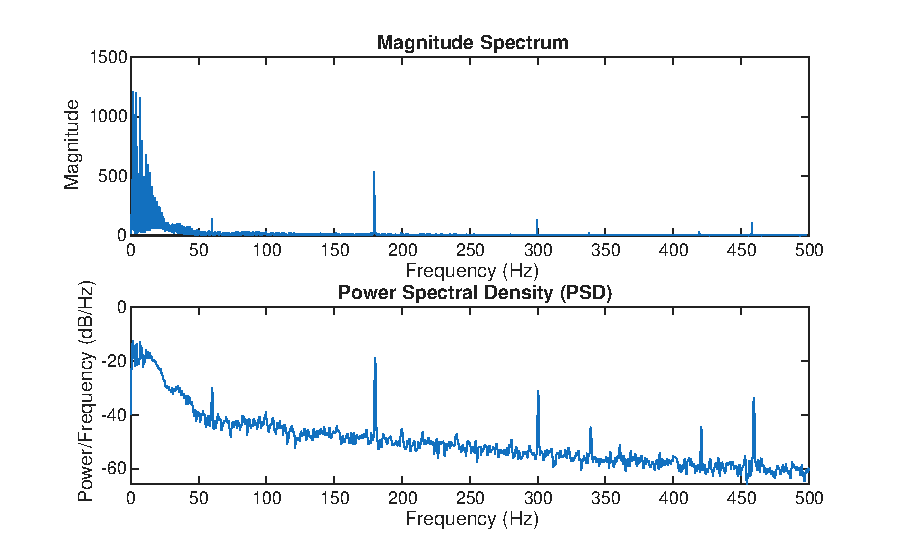
\includegraphics[width=\maxwidth{56.196688409433015em}]{figure_5.eps}
\end{center}

\begin{par}
\begin{flushleft}
There can be observed 4 clear and distinctive peaks offside the frequency values of the ECG (at 60, 180, 300, 460 Hz). These peaks are caused by electric interferences of the medical device used to record the ECG. The 60Hz frequency peak is due to the electrical plug where the device is connected (in USA is 60Hz). The other peaks are resulting from the harmonics of the plug frequency.
\end{flushleft}
\end{par}

\matlabheadingthree{Type of filter to apply}

\begin{par}
\begin{flushleft}
Seeing that the data has peaks (from noise from 60Hz upside), we could use a:
\end{flushleft}
\end{par}

\begin{itemize}
\setlength{\itemsep}{-1ex}
   \item{\begin{flushleft} Low pass filter from somewhere around 40 - 50Hz. \end{flushleft}}
   \item{\begin{flushleft} Zero phase filter (filtfilt) to avoid phase shift. \end{flushleft}}
\end{itemize}


\matlabheadingtwo{2.3. Apply selected filter (order 4)}

\begin{par}
\begin{flushleft}
A low pass filter, eliminates the compounds of the signal oscilating above a threshold. For this case we will calculate the filter coeficients with the function "butter", and will filter the signal with the function filtfilt.
\end{flushleft}
\end{par}

\begin{matlabcode}
% Apply built in low pass filter
[b,a] = butter(4, 40/(fs/2), 'low');  % diseño del filtro
ecgff = filtfilt(b, a, ecgf);
samples_to_plot = 1:1400;

figure;
hold on;
plot(time(samples_to_plot), ecgf(samples_to_plot));
plot(time(samples_to_plot), ecgff(samples_to_plot));

legend('Raw signal', 'Filtered Signal')
title('Raw and filtered ecg signal')
\end{matlabcode}
\begin{center}
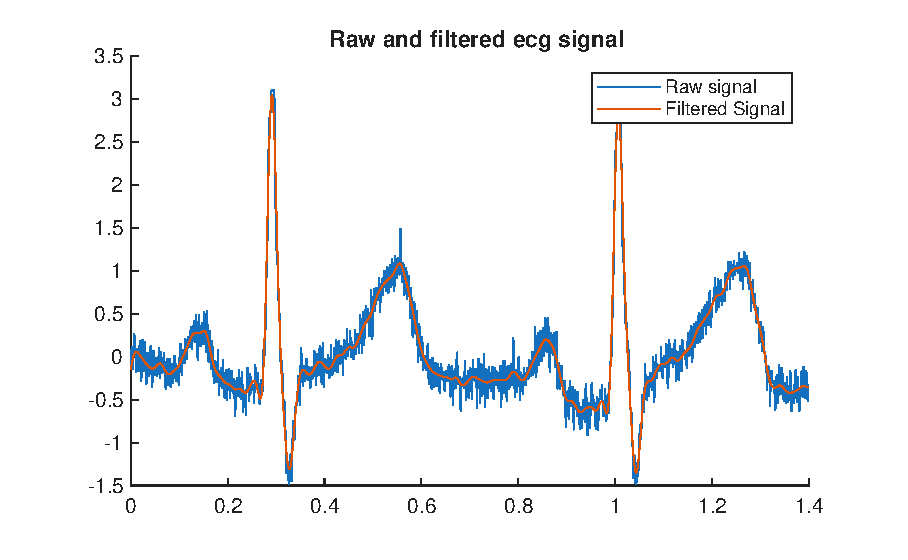
\includegraphics[width=\maxwidth{56.196688409433015em}]{figure_6.eps}
\end{center}

\begin{par}
\begin{flushleft}
As it can be seen, the resulting signal only contains shape of the ECG, and all that high frequency components are eliminated.
\end{flushleft}
\end{par}

\matlabheadingtwo{2.3. Compare before and after filtering}

\begin{par}
\begin{flushleft}
Now, we can see the resulting frequencies that live in our filtered signal. 
\end{flushleft}
\end{par}

\begin{matlabcode}
% Take the magnitude spectrum
[magnitudef, ff] = magnitude_spectrum(ecgff, fs);
% Compute PSD using Welch's method
[pxxf, f_psdf] = pwelch(ecgff, [], [], [], fs);

figure;

% FFT Magnitude
subplot(2,1,1);
hold on;
plot(f, magnitude);
plot(ff, magnitudef);
xlabel('Frequency (Hz)');
ylabel('Magnitude');
title('Magnitude Spectrum');
legend('Raw', 'Filtered');

% PSD
subplot(2,1,2);
hold on;
plot(f_psd, 10*log10(pxx));  % PSD in dB/Hz
plot(f_psdf, 10*log10(pxxf));  % PSD in dB/Hz
xlabel('Frequency (Hz)');
ylabel('Power/Frequency (dB/Hz)');
title('Power Spectral Density (PSD)');
legend('Raw', 'Filtered');
\end{matlabcode}
\begin{center}
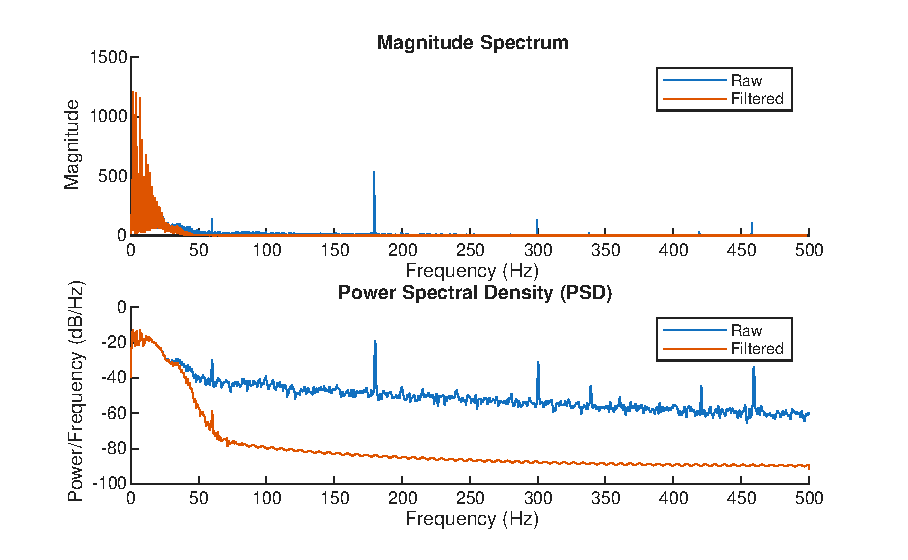
\includegraphics[width=\maxwidth{56.196688409433015em}]{figure_7.eps}
\end{center}

\begin{par}
\begin{flushleft}
As those oscillations were removed by the low pass filter, the peaks over 40HZ are not present any more. Which further confirms that our signal is correctly filtered.
\end{flushleft}
\end{par}


\matlabheadingtwo{2.4. Filer Twave}

\begin{par}
\begin{flushleft}
In this section we need to filter the T-wave component of our ECG.
\end{flushleft}
\end{par}

\begin{par}
\begin{flushleft}
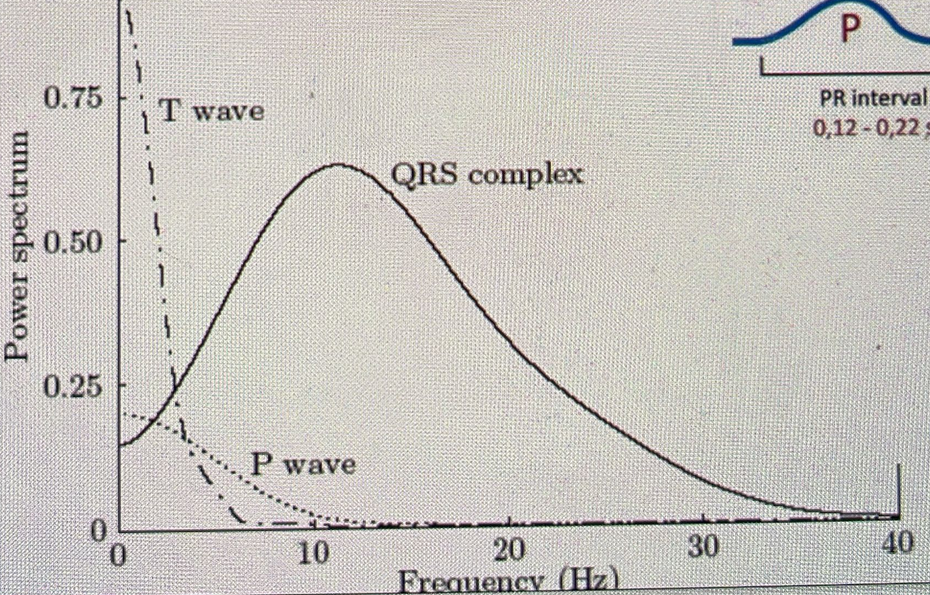
\includegraphics[width=\maxwidth{53.487205218263924em}]{image_2}
\end{flushleft}
\end{par}

\begin{par}
\begin{flushleft}
This plot shows the frequency range that each wave in the ECG has. If we look closely, we can see the following:
\end{flushleft}
\end{par}

\begin{itemize}
\setlength{\itemsep}{-1ex}
   \item{\begin{flushleft} T wave 0 \textasciitilde{} 7 Hz \end{flushleft}}
   \item{\begin{flushleft} P wave 0 \textasciitilde{} 14 Hz \end{flushleft}}
   \item{\begin{flushleft} QRS complex 0 \textasciitilde{} 40 Hz (but predominant in \textasciitilde{} 13 Hz) \end{flushleft}}
\end{itemize}

\begin{par}
\begin{flushleft}
With this information, we can conclude that the ideal filter could be a \textasciitilde{}5Hz highpass filter. This would remove the predominant frequencies of the T wave, while mantaining the other complexes mostly intact.
\end{flushleft}
\end{par}

\begin{matlabcode}
% Find the frequency of the T-wave and filter it from the signal
freq_limit = 5;
[b,a] = butter(4, freq_limit/(fs/2), "high");
filtered_t_waves = filtfilt(b, a, ecgff);
samples_to_plot = 1:1400;

figure;
hold on;
plot(time(samples_to_plot), filtered_t_waves(samples_to_plot));
plot(time(samples_to_plot), ecgff(samples_to_plot));
xlabel('Time (s)');
ylabel('Amplitude (mV)');
title('Filtered T wave');
\end{matlabcode}
\begin{center}
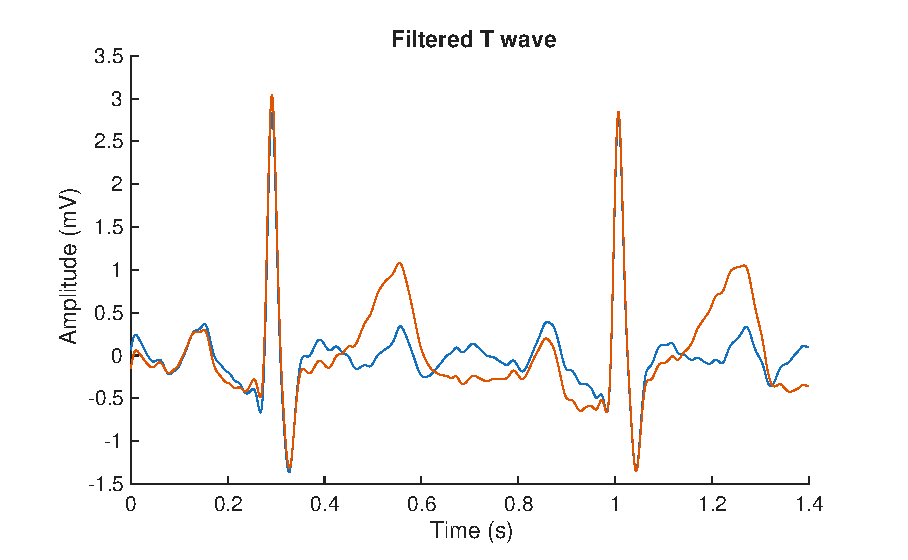
\includegraphics[width=\maxwidth{56.196688409433015em}]{figure_8.eps}
\end{center}

\begin{par}
\begin{flushleft}
The T-waves are notably reduced, and the other components remain nearly the same. After some trials, we can conclude that the 5Hz highpass is the sweetpoint for this purpose.
\end{flushleft}
\end{par}


\matlabheadingtwo{2.5. Filter comparison Zero Phase vs IIR}

\begin{matlabcode}
freq_limit = 5;        % cutoff in Hz 
[b_iir,a_iir] = butter(4, freq_limit/(fs/2), 'high'); % 4th-order highpass Butterworth

% Apply single-pass IIR and double-pass (zero-phase)
ecg_iir_single = filter(b_iir, a_iir, ecgff);    % single pass (causes phase distortion)
ecg_iir_filtfilt = filtfilt(b_iir, a_iir, ecgff);% zero-phase double-pass

% Time-domain overlay (zoom window)
samples_to_plot = 1:1400; % as you used, adjust if needed
figure;
plot(time(samples_to_plot), ecgff(samples_to_plot), 'DisplayName','original ecgff'); hold on;
plot(time(samples_to_plot), ecg_iir_single(samples_to_plot), '--', 'DisplayName','IIR single-pass');
plot(time(samples_to_plot), ecg_iir_filtfilt(samples_to_plot), '-.', 'DisplayName','IIR filtfilt (zero-phase)');
xlabel('Time (s)'); ylabel('Amplitude (mV)');
title('ECG: original vs IIR filtered (single-pass and filtfilt)');
legend; grid on;
\end{matlabcode}
\begin{center}
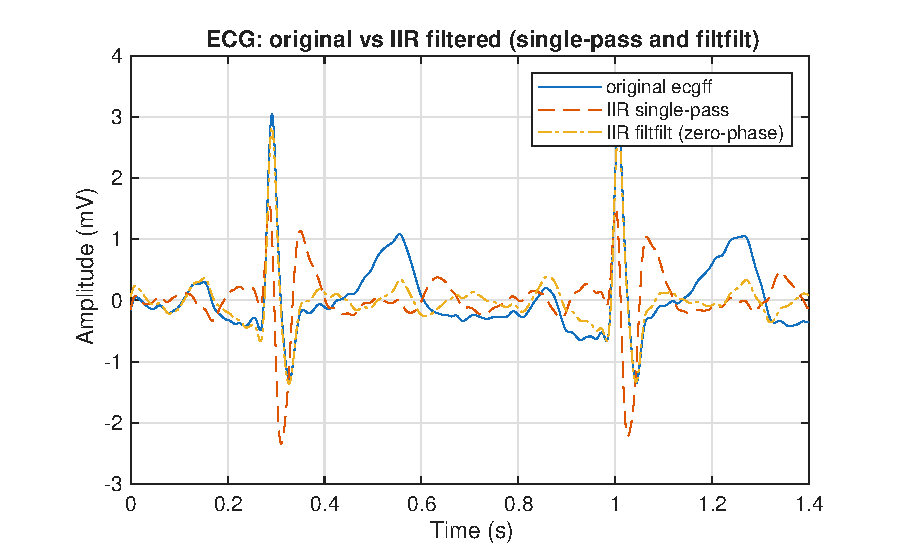
\includegraphics[width=\maxwidth{56.196688409433015em}]{figure_9.eps}
\end{center}

\begin{par}
\begin{flushleft}
The single-pass filter, in this case filters better the T-wave, however, it also filters considerably the QRS complex. The zero-phase filtfilt leaves the QRS complex barely untouched.
\end{flushleft}
\end{par}

\begin{par}
\begin{flushleft}
This is due to the effect of the zero-phase filtering, as it runs the filter \textit{forward} and then \textit{backward, }\textbf{canceling the phase shift} introduced in the forward pass.
\end{flushleft}
\end{par}

\matlabheadingthree{Compare filtered signals and their PSD}

\begin{par}
\hfill \break
\end{par}

\begin{matlabcode}
nfft = 4096;
win = round(0.5*fs);
noverlap = round(0.25*fs);
[Px_orig,f_orig] = pwelch(ecgff, win, noverlap, nfft, fs);
[Px_single,f_single] = pwelch(ecg_iir_single, win, noverlap, nfft, fs);
[Px_filtfilt,f_filtfilt] = pwelch(ecg_iir_filtfilt, win, noverlap, nfft, fs);

figure;
plot(f_orig, 10*log10(Px_orig), 'DisplayName','original'); hold on;
plot(f_single, 10*log10(Px_single), '--', 'DisplayName','IIR single-pass');
plot(f_filtfilt, 10*log10(Px_filtfilt), '-.', 'DisplayName','IIR filtfilt');
xlim([0 60]); % zoom to relevant ECG band
xlabel('Frequency (Hz)'); ylabel('PSD (dB/Hz)');
title('PSD: original vs IIR filtered');
legend; grid on;
\end{matlabcode}
\begin{center}
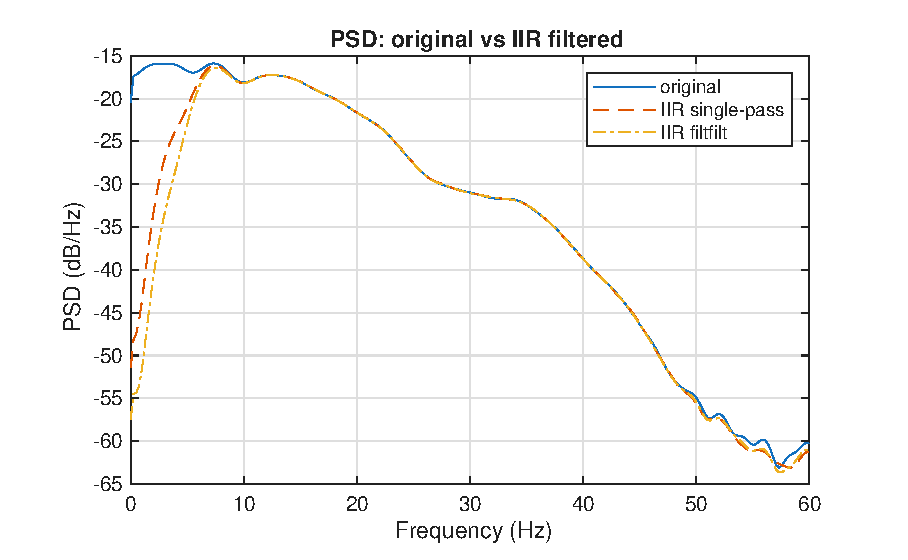
\includegraphics[width=\maxwidth{56.196688409433015em}]{figure_10.eps}
\end{center}


\matlabheadingtwo{2.6. Filter Order Increasing}

\begin{par}
\begin{flushleft}
In this exercise, we will compare IIR and FIR filters. IIR filt filt method achieves good filtering of the signal. However, a FIR filter with a defined order can be engineered to match the output of the IIR filter.
\end{flushleft}
\end{par}

\begin{par}
\begin{flushleft}
In this exercise we will:
\end{flushleft}
\end{par}

\begin{itemize}
\setlength{\itemsep}{-1ex}
   \item{\begin{flushleft} Get the target\_reduction\_dB obtained by the IIR implementation over the signal. \end{flushleft}}
   \item{\begin{flushleft} Search for the FIR order that results the most similar to the IIR filter. \end{flushleft}}
\end{itemize}

\begin{matlabcode}

% Numeric metric: energy below 6 Hz (T-wave band)
T_band = [0 6];
orig_T_energy = bandpower(ecgff, fs, T_band);
single_T_energy = bandpower(ecg_iir_single, fs, T_band);
filtfilt_T_energy = bandpower(ecg_iir_filtfilt, fs, T_band);
fprintf('T-band energy reduction (dB): single-pass = %.2f dB, filtfilt = %.2f dB\n', ...
    10*log10(single_T_energy/orig_T_energy), 10*log10(filtfilt_T_energy/orig_T_energy));
\end{matlabcode}
\begin{matlaboutput}
T-band energy reduction (dB): single-pass = -9.24 dB, filtfilt = -13.02 dB
\end{matlaboutput}
\begin{matlabcode}

%% FIR comparison: start with order 4, then sweep orders to match filtfilt attenuation
orders = [4 8 16 32 64 128 256 512]; % pick candidates; adjust to your computation time
best_order = NaN; best_diff = Inf;
target_reduction_dB = 10*log10(filtfilt_T_energy/orig_T_energy); % negative number

fprintf('Target T-band reduction (IIR filtfilt): %.2f dB\n', target_reduction_dB);
\end{matlabcode}
\begin{matlaboutput}
Target T-band reduction (IIR filtfilt): -13.02 dB
\end{matlaboutput}
\begin{matlabcode}

for ord = orders
    % Design linear-phase FIR highpass
    b_fir = fir1(ord, freq_limit/(fs/2), 'high'); 
    ecg_fir = filtfilt(b_fir, 1, ecgff); % zero-phase FIR (recommended so no delay)
    
    % Compute PSD & T-band energy
    fir_T_energy = bandpower(ecg_fir, fs, T_band);
    fir_reduction_dB = 10*log10(fir_T_energy / orig_T_energy);
    fprintf('FIR order %3d -> T-band reduction: %.2f dB\n', ord, fir_reduction_dB);
    
    diff = abs(fir_reduction_dB - target_reduction_dB);
    if diff < best_diff
        best_diff = diff; 
        best_order = ord; best_ecg_fir = ecg_fir; 
        best_fir_reduction = fir_reduction_dB;
    end
end
\end{matlabcode}
\begin{matlaboutput}
FIR order   4 -> T-band reduction: -0.38 dB
FIR order   8 -> T-band reduction: -0.77 dB
FIR order  16 -> T-band reduction: -1.56 dB
FIR order  32 -> T-band reduction: -3.24 dB
FIR order  64 -> T-band reduction: -6.84 dB
FIR order 128 -> T-band reduction: -13.73 dB
FIR order 256 -> T-band reduction: -17.83 dB
FIR order 512 -> T-band reduction: -17.88 dB
\end{matlaboutput}
\begin{matlabcode}

fprintf('Best matching FIR order: %d (reduction %.2f dB, diff %.2f dB)\n', best_order, best_fir_reduction, best_diff);
\end{matlabcode}
\begin{matlaboutput}
Best matching FIR order: 128 (reduction -13.73 dB, diff 0.71 dB)
\end{matlaboutput}
\begin{matlabcode}

% Plot best FIR vs IIR filtfilt and original (time zoom)
figure;
plot(time(samples_to_plot), ecgff(samples_to_plot), 'DisplayName','original'); hold on;
plot(time(samples_to_plot), ecg_iir_filtfilt(samples_to_plot), '--', 'DisplayName','IIR filtfilt');
plot(time(samples_to_plot), best_ecg_fir(samples_to_plot), '-.', 'DisplayName', sprintf('FIR order %d', best_order));
xlabel('Time (s)'); ylabel('Amplitude (mV)');
title(sprintf('Best FIR (order %d) vs IIR filtfilt (time domain)', best_order));
legend; grid on;
\end{matlabcode}
\begin{center}
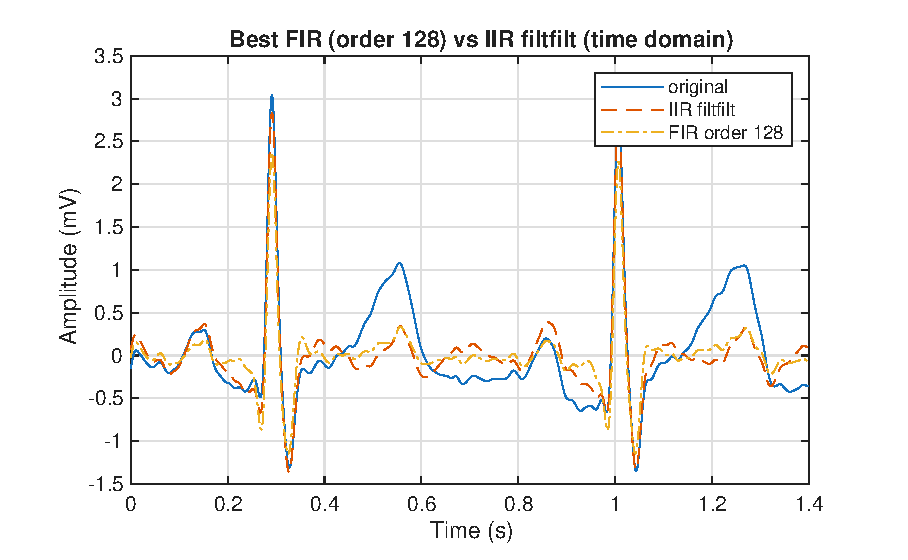
\includegraphics[width=\maxwidth{56.196688409433015em}]{figure_11.eps}
\end{center}

\begin{par}
\begin{flushleft}
As it can be seen, the best matching order against filtfilt method is 128. This order makes that the filter output of both are the most similar possible among the different orders.
\end{flushleft}
\end{par}

\begin{matlabcode}

% PSD overlay for best FIR
[Px_fir, f] = pwelch(best_ecg_fir, win, noverlap, nfft, fs);
figure;
plot(f,10*log10(Px_orig), 'DisplayName','original'); hold on;
plot(f,10*log10(Px_filtfilt),'--','DisplayName','IIR filtfilt');
plot(f,10*log10(Px_fir),'-.','DisplayName', sprintf('FIR ord %d', best_order));
xlim([0 60]); xlabel('Frequency (Hz)'); ylabel('PSD (dB/Hz)');
title('PSD: original vs IIR filtfilt vs best FIR'); legend; grid on;
\end{matlabcode}
\begin{center}
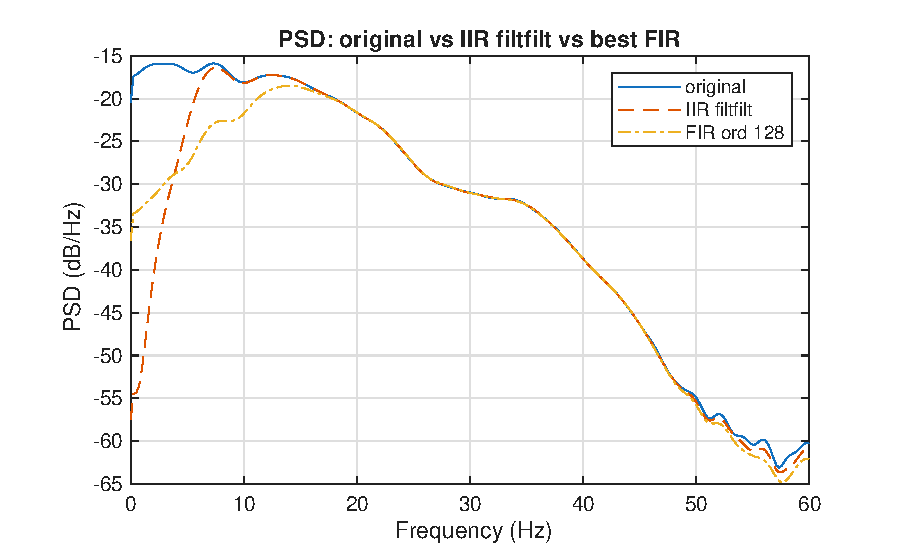
\includegraphics[width=\maxwidth{56.196688409433015em}]{figure_12.eps}
\end{center}

\begin{par}
\begin{flushleft}
The FIR PSD is slightly different, and will filter frequencies up to 15Hz, whereas the IIR filtfilt method is cleaner and adapts better to the signal.
\end{flushleft}
\end{par}

\end{document}
